
\chapter{Chapter 1. Introduction}%Be sure to include Chapter 1. before you write the name of your chapter. Name all remaining chapters in the same manner.

\section{Formatting}

Chapter titles should begin with the word chapter and the appropriate number followed by a period. After typing the chapter heading, then type the chapter title. This template automatically formats your chapter titles. Just do not forget to include the chapter heading when you type the chapter name.

All paragraphs throughout your thesis should begin with an ½ inch indentation. It should be double-spaced throughout. Since this is a formal document, do not use contractions. Remember that paragraphs should consist of at least two sentences. Figure 1.1 lists 11 common grammar mistakes. Please avoid these!
\begin{figure}[ht]
    \centering
    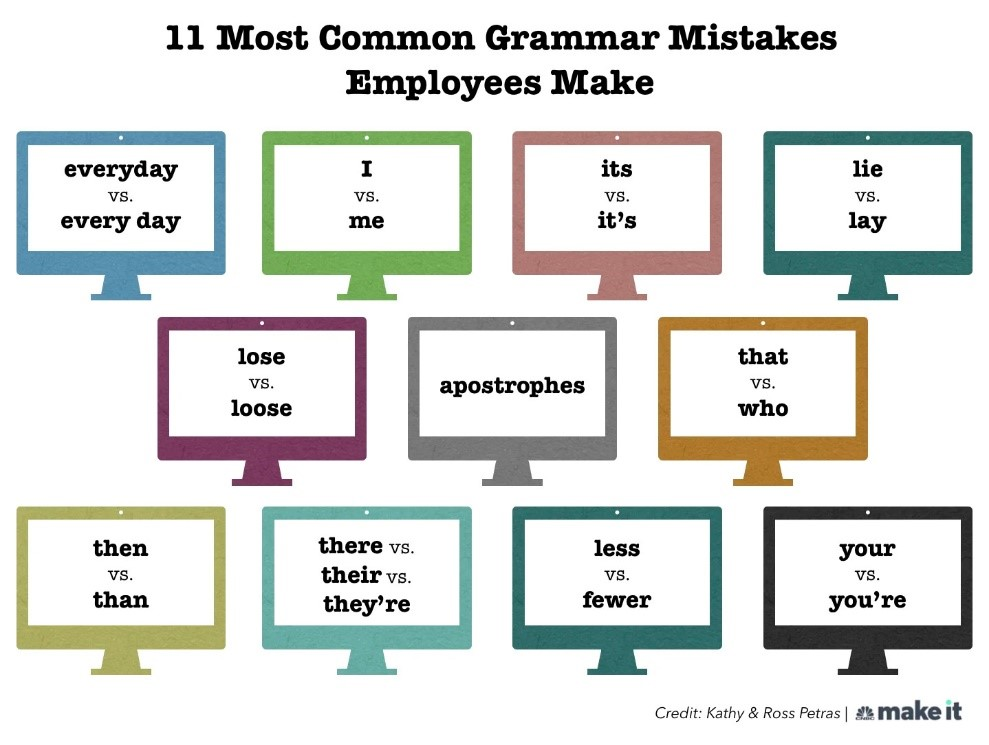
\includegraphics[scale=.7]{Figures/figure 1.1.jpg}
    \caption[11 Most Common Grammar Mistakes Employees Make: I'm purposely making this longer to extend to two lines.]{11 Most Common Grammar Mistakes Employees Make. When labeling your figures, single-space if captions extend to two lines}
    \label{fig 1.1}
\end{figure}

\section{Symbols}

If your document includes many symbols or acronyms, you may include a List of Symbols, Abbreviations, \textit{etc}. If you want a symbol/abbreviation included in the List of Symbols, be sure to create an entry for it first on the List of Symbols Glossaries.tex file. Once it is created, then you can insert it with a glossaries command. For example, the current temperature outside is 100\glspl{deg}.

You can capitalize your symbols or make them plural by using different commands included with the glossaries package. However, only those symbols that are actually referenced in the body of your thesis will be present in the List of Symbols. Below are a few more symbol examples.

\gls{grav}

\gls{wf}

\gls{alp}

\gls{theta}

\gls{te}

\gls{q10}

\gls{phi}

